\documentclass[a4paper]{article}

\usepackage[english]{babel}
\usepackage[utf8]{inputenc}
\usepackage{amsmath}
\usepackage{graphicx}
\usepackage[colorinlistoftodos]{todonotes}

\usepackage{pdfpages}

\title{Small World : Rapport de Modélisation}

\author{Axel CARO, Maximilien RICHER}

\date{\today}

\begin{document}
\maketitle

\paragraph{}
Ce document présente les résultats de la phase de modélisation du projet de quatrième année proposé en enseignement de \textit{Programmation et Modélisation orientées objet}.

\section{Introduction}
Bla bla le projet.

\section{Modélisation UML}
La phase de modélisation nous a conduit à réaliser plusieurs diagrammes UML, afin de représenter différents aspects de notre application. Nous présentons ci-après ces diagrammes, en explicitant leur contenu.

\subsection{Diagramme de paquetage}
\paragraph{}
Le diagramme suivant illustre la structuration à gros grain du code de notre application. On y retrouve les classes et interfaces que nous détaillerons dans la section \ref{DDC}. Ce diagramme illustre les interactions entre les regroupements de classes. On ne parle pas ici de \textit{package} proprement dit, car le choix du \textbf{C\#} comme langage de programmation ne permet pas l'utilisation de paquetages. Il s'agit d'un découpage ayant pour but de présenter la structure des différentes parties de l'application, sans détailler les interactions internes à chaque regroupement.

\paragraph{}
On distingue 7 regroupements, en plus de l'application principale (\textit{SmallWorld}) :
\begin{enumerate}
\item \textit{Tile} : gestion des cases du terrain de jeu.
\item \textit{Map} : gestion du terrain de jeu.
\item \textit{Race} : gestion des différentes races jouables.
\item \textit{Unit} : gestion des unités.
\item \textit{Player} : gestion des joueurs.
\item \textit{Game} : gestion de la partie.
\item \textit{SaveLoad} : gestion de la sauvegarde et du chargement de parties.
\end{enumerate}

\paragraph{}
Les interactions entre ces différents regroupements sont symbolisées par les flèches présentes sur le diagramme. Par exemple, le groupement \textit{Map} utilise des membres du groupement \textit{Tile}. Les interactions ainsi mises en valeur présentent bien la mise en cascade des regroupements, selon les données modélisées.

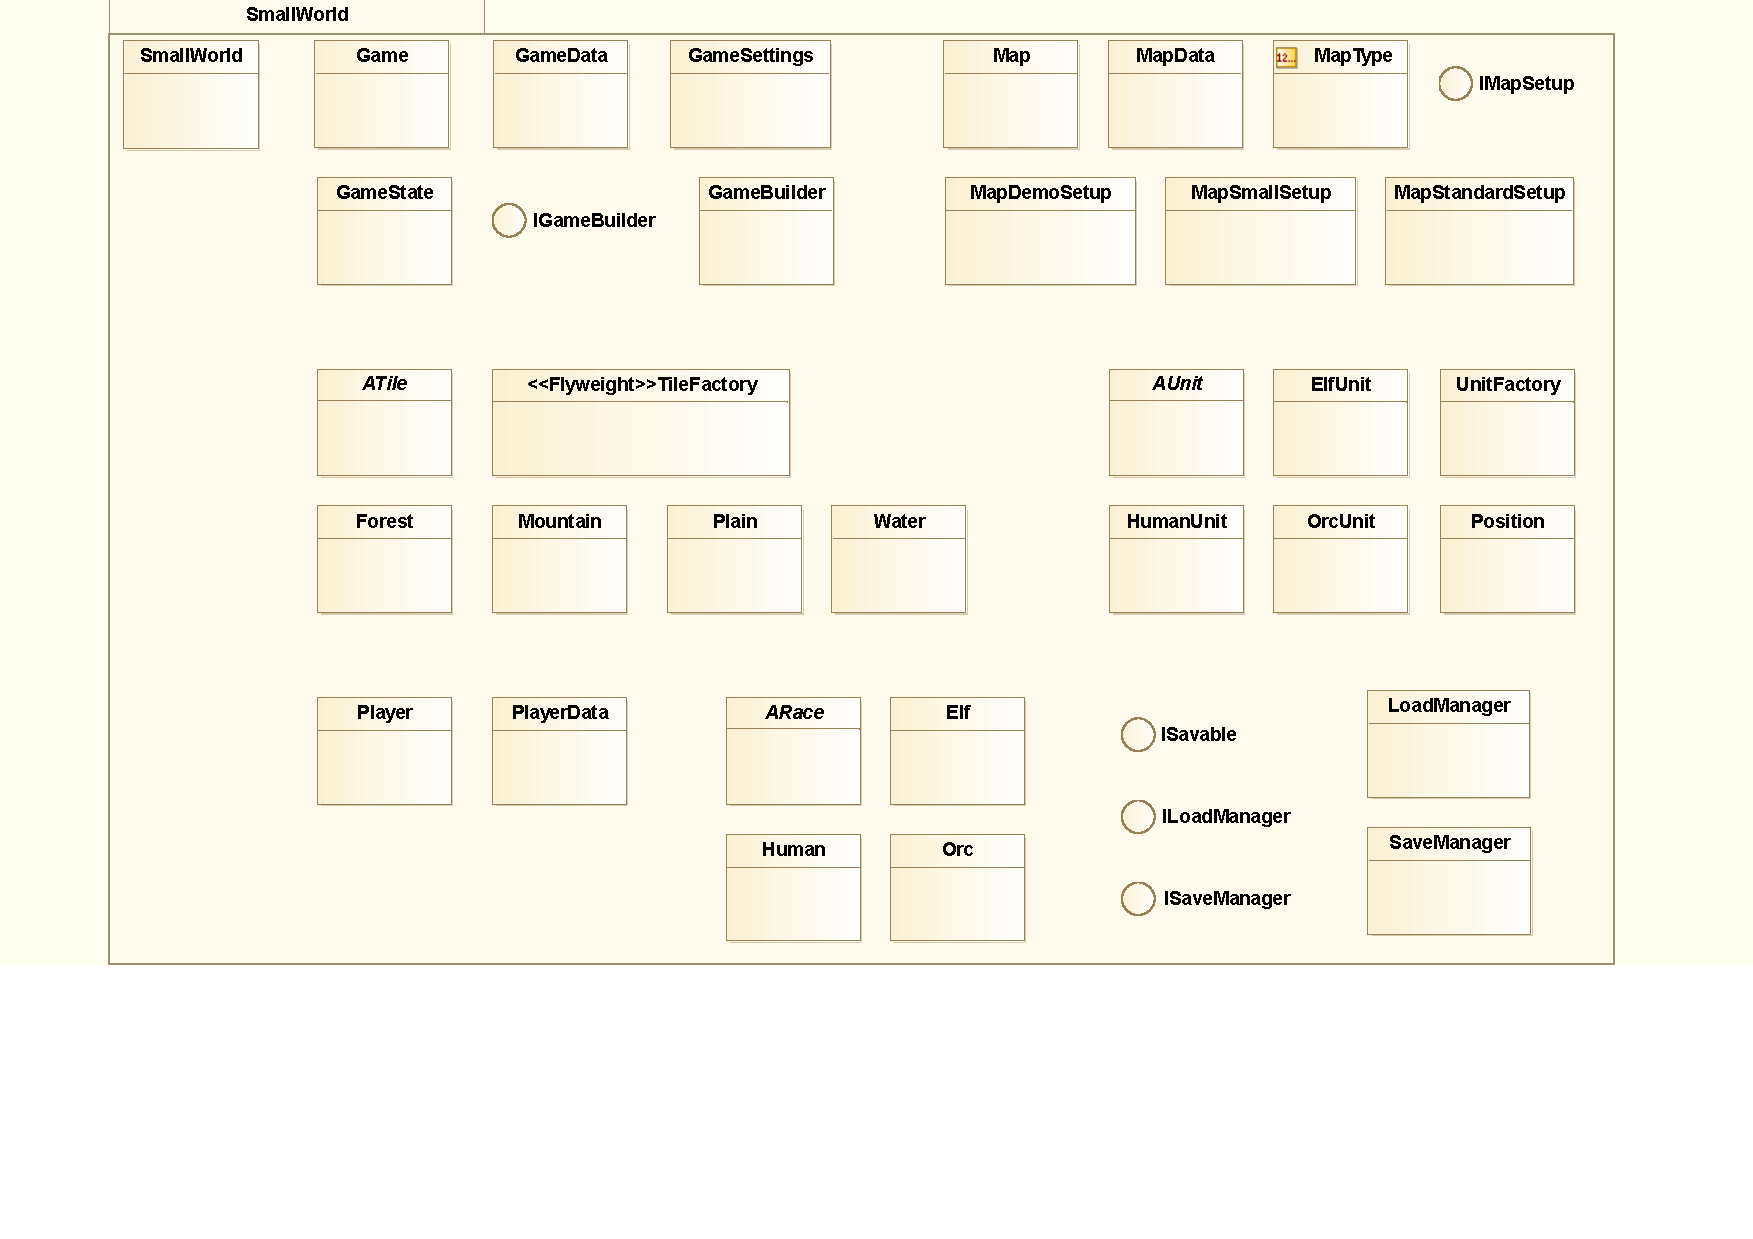
\includepdf[landscape=true]{images/packageDiagram.pdf}

\subsection{Diagramme de classes}
\label{DDC}

\subsection{Diagrammes d'interaction}

\subsubsection{Diagramme de séquence : initialisation d'une partie}

\subsubsection{Diagramme de séquence : déroulement d'un tour}

\subsection{Diagramme d'états-transitions : gestion d'une unité}

\end{document}